\documentclass[11pt,a4paper]{article}

\usepackage[margin=1.85cm]{geometry}
\usepackage[T1]{fontenc}
\usepackage[utf8]{inputenc}
\usepackage{lmodern}
\usepackage{microtype}
\usepackage{amsmath,amssymb}
\usepackage{booktabs}
\usepackage{array}
\usepackage{tabularx}
\usepackage{longtable}
\usepackage{graphicx}
\usepackage{float}
\usepackage{enumitem}
\usepackage{xcolor}
\usepackage{hyperref}
\usepackage{listings}
\usepackage{tikz}

\usetikzlibrary{arrows.meta, positioning, calc}

\hypersetup{
  colorlinks=true,
  linkcolor=blue!45!black,
  urlcolor=teal!50!black,
  pdftitle={Retrieval Engine Competition Project - Notebook-Aligned Report},
  pdfauthor={Maksym DOLHOV; Mehdi AGHAEI; Nguyen Ho Bao KHANH},
  pdfsubject={SeaFour notebook-aligned retrieval report}
}

\definecolor{ink}{HTML}{233648}
\definecolor{accent}{HTML}{2A6F97}
\definecolor{softblue}{HTML}{EAF3FA}
\definecolor{softgreen}{HTML}{E9F5EE}
\definecolor{softgold}{HTML}{F7F1D8}
\definecolor{softgray}{HTML}{F4F6F8}
\definecolor{rulegray}{HTML}{D6DCE3}

\setlength{\parindent}{0pt}
\setlength{\parskip}{5.5pt}
\renewcommand{\arraystretch}{1.18}
\setlist[itemize]{leftmargin=1.4em, itemsep=2pt, topsep=3pt}
\setlist[enumerate]{leftmargin=1.5em, itemsep=2pt, topsep=3pt}

\lstdefinestyle{codeblock}{
  basicstyle=\ttfamily\footnotesize,
  breaklines=true,
  columns=fullflexible,
  keepspaces=true,
  frame=single,
  framesep=4pt,
  framerule=0.4pt,
  rulecolor=\color{rulegray},
  backgroundcolor=\color{softgray}
}
\lstset{style=codeblock}

\newcommand{\metric}[1]{\textbf{#1}}
\newcommand{\smallcaps}[1]{\textsc{#1}}
\newcolumntype{Y}{>{\raggedright\arraybackslash}X}

\begin{document}

\begin{titlepage}
\centering
\vspace*{1.0cm}

{\Large\bfseries Retrieval Engine Competition Project\par}
\vspace{0.2cm}
{\large Notebook Report\par}
\vspace{0.6cm}
{\large Group: SeaFour\par}
\vspace{0.9cm}

\begin{tabular}{c}
Maksym DOLHOV \\
Mehdi AGHAEI \\
Nguyen Ho Bao KHANH \\
\end{tabular}

\vspace{1.0cm}

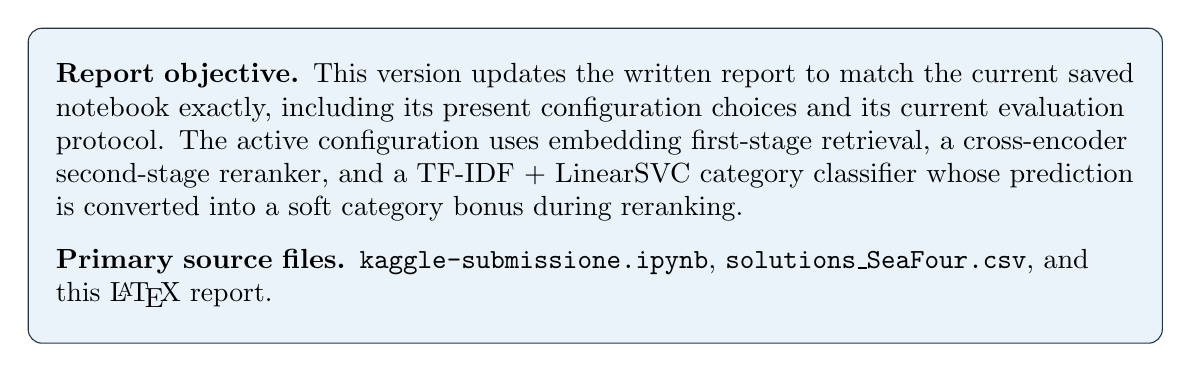
\begin{tikzpicture}[x=1cm,y=1cm,>=Latex]
  \node[draw=ink, rounded corners=5pt, fill=softblue, text width=13.7cm, minimum height=4.0cm, align=left, inner sep=10pt] (box) at (0,0) {
  \textbf{Report objective.} This version updates the written report to match the current saved notebook exactly, including its present configuration choices and its current evaluation protocol. The active configuration uses embedding first-stage retrieval, a cross-encoder second-stage reranker, and a TF-IDF + LinearSVC category classifier whose prediction is converted into a soft category bonus during reranking.\\[0.25cm]
  \textbf{Primary source files.} \texttt{kaggle-submissione.ipynb}, \texttt{solutions\_SeaFour.csv}, and this \LaTeX\ report.};
\end{tikzpicture}

\vspace{0.8cm}

\begin{tabular}{>{\bfseries}p{0.27\linewidth}p{0.60\linewidth}}
Notebook file & \texttt{kaggle-submissione.ipynb} \\
Submission file & \texttt{solutions\_SeaFour.csv} \\
Current default model & \texttt{embedding} \\
Submission size target & Top 7,500 first-stage candidates; offline rerank top 150; submission cell reranks top 20 \\
Date & \today \\
\end{tabular}

\vfill
\end{titlepage}

\section{Notebook-Aligned System Overview}

The logic is organized into several stages: strict data loading, shared text normalization, sequential model experimentation (TF-IDF to BM25+ to embeddings), aggressive caching for performance, category-classifier fitting, cross-encoder training, offline evaluation on the training queries, and final submission generation.

The current system relies on a dense first-stage embedding retriever followed by a cross-encoder reranker, with category information injected as a soft bonus.

The present notebook snapshot is configured as follows:
\begin{itemize}
    \item \texttt{EVALUATION\_TOP\_KS = [7500]}
    \item \texttt{CROSS\_ENCODER\_TRAIN\_QUERY\_LIMIT = 327}
    \item \texttt{CROSS\_ENCODER\_RERANK\_TOP\_M = 150} for offline evaluation
    \item category bonus \(= 2.0\) whenever \texttt{ENABLE\_CATEGORY\_FILTER = True}
    \item the test-submission cell overrides the reranking depth to \texttt{top\_m = 20}
\end{itemize}

\begin{figure}[H]
\centering
\resizebox{1.0\linewidth}{!}{%
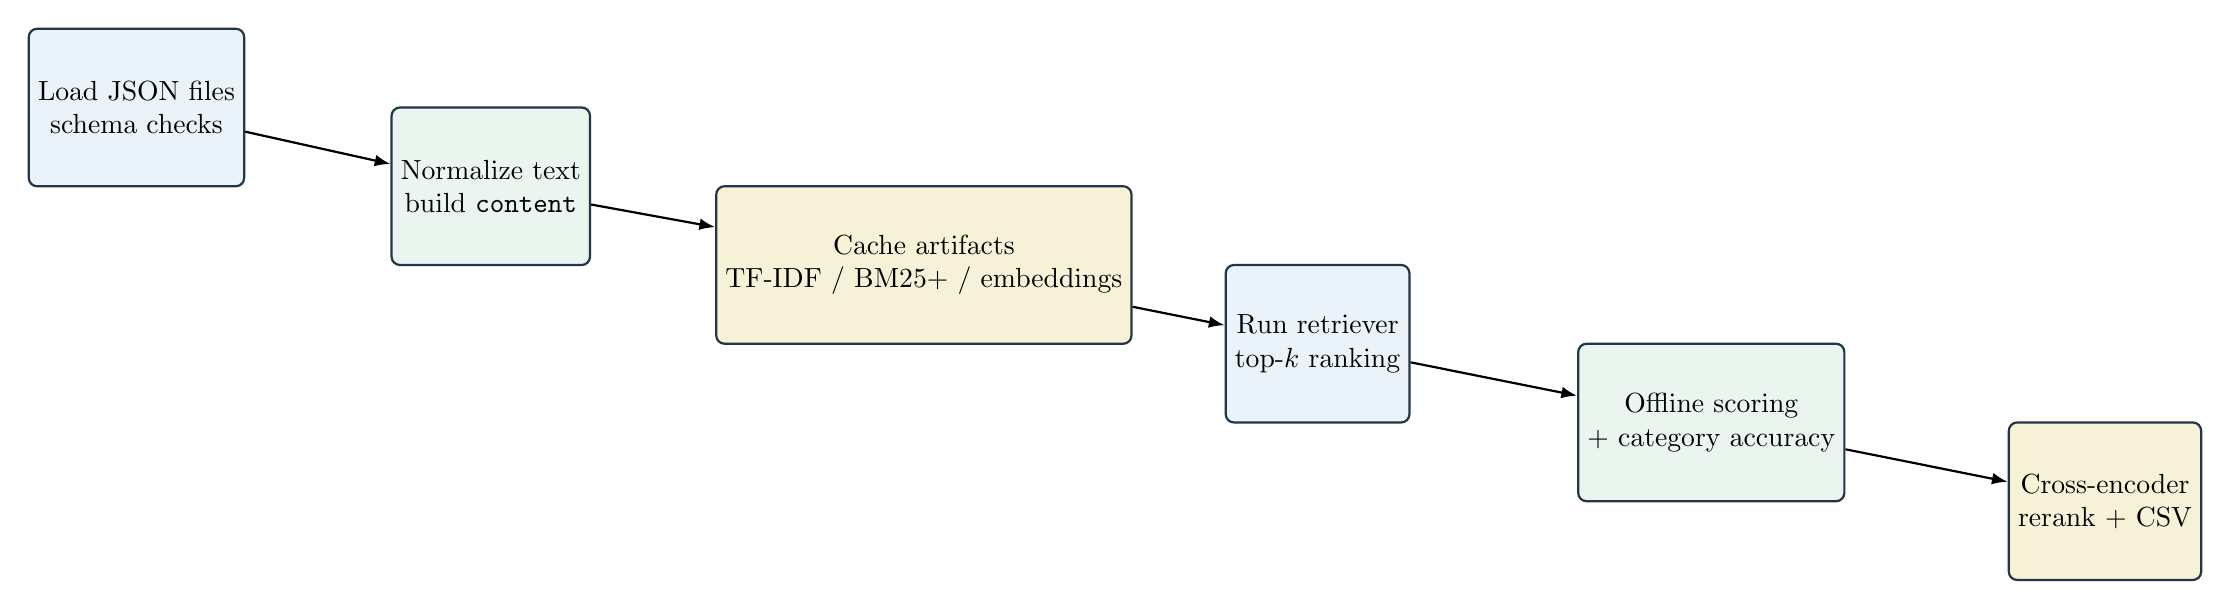
\begin{tikzpicture}[
  box/.style={draw=ink, rounded corners=3pt, minimum width=1cm, minimum height=2cm, align=center, thick},
  >={Latex[length=2.0mm]}
]
\node[box, fill=softblue]   (data)   at (-5,5)    {Load JSON files\\schema checks};
\node[box, fill=softgreen]  (prep)   at (-0.5,4) {Normalize text\\build \texttt{content}};
\node[box, fill=softgold]   (index)  at (5.0,3) {Cache artifacts\\TF-IDF / BM25+ / embeddings};
\node[box, fill=softblue]   (retr)   at (10.0,2){Run retriever\\top-$k$ ranking};
\node[box, fill=softgreen]  (eval)   at (15.0,1){Offline scoring\\+ category accuracy};
\node[box, fill=softgold]   (sub)    at (20.0,0){Cross-encoder\\rerank + CSV};

\draw[->, thick] (data) -- (prep);
\draw[->, thick] (prep) -- (index);
\draw[->, thick] (index) -- (retr);
\draw[->, thick] (retr) -- (eval);
\draw[->, thick] (eval) -- (sub);
\end{tikzpicture}}
\caption{Active end-to-end workflow in the saved notebook.}
\end{figure}

\begin{table}[H]
\centering
\small
\begin{tabularx}{\linewidth}{>{\bfseries}l c c Y}
\toprule
Component & Implemented & Active in saved run & Role in the pipeline \\
\midrule
TF-IDF retrieval & Yes & No & Sparse lexical baseline using cosine similarity. Fast, but struggled with semantic mismatch. \\
BM25+ retrieval & Yes & No & Stronger lexical baseline with token-level scoring and document-length normalization. \\
Embedding retrieval & Yes & Yes & Dense semantic first-stage retrieval with Sentence-Transformers. Yielded the best metrics. \\
Cross-encoder reranker & Yes & Yes & Re-ranks the first-stage candidates using joint query-document scoring. The current notebook uses top-\(m=150\) during offline evaluation and top-\(m=20\) in the submission cell. \\
Category classifier & Yes & Yes & Predicts one category per query, reports train-query accuracy, and provides a soft category bonus of \(2.0\) during reranking when enabled. \\
Dominant-category strict filter & Yes & No & Kept as an implemented option, but disabled in the active saved run. \\
\bottomrule
\end{tabularx}
\caption{What the notebook supports versus what the saved execution actually uses.}
\end{table}

\section{Dataset and Preprocessing}

The notebook loads 216,041 documents, 327 training queries, 141 test queries, and one training qrels file. The document collection is distributed across five categories, with significant class imbalance.

\begin{figure}[H]
\centering
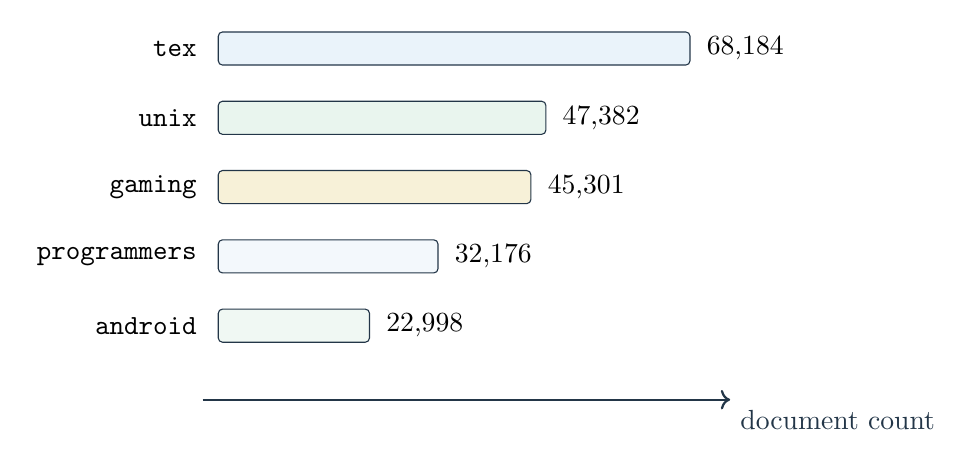
\begin{tikzpicture}[x=1cm,y=1cm]
\draw[->, thick, color=ink] (0,0.55) -- (6.7,0.55) node[below right] {document count};
\filldraw[fill=softblue, draw=ink, rounded corners=1.5pt]  (0.20,4.80) rectangle (6.19,5.22);
\node[anchor=east] at (0.05,5.01)  {\texttt{tex}};
\node[anchor=west] at (6.28,5.01)  {68,184};
\filldraw[fill=softgreen, draw=ink, rounded corners=1.5pt] (0.20,3.92) rectangle (4.36,4.34);
\node[anchor=east] at (0.05,4.13)  {\texttt{unix}};
\node[anchor=west] at (4.45,4.13)  {47,382};
\filldraw[fill=softgold, draw=ink, rounded corners=1.5pt]  (0.20,3.04) rectangle (4.17,3.46);
\node[anchor=east] at (0.05,3.25)  {\texttt{gaming}};
\node[anchor=west] at (4.26,3.25)  {45,301};
\filldraw[fill=softblue!55, draw=ink, rounded corners=1.5pt] (0.20,2.16) rectangle (2.99,2.58);
\node[anchor=east] at (0.05,2.37)  {\texttt{programmers}};
\node[anchor=west] at (3.08,2.37)  {32,176};
\filldraw[fill=softgreen!70, draw=ink, rounded corners=1.5pt] (0.20,1.28) rectangle (2.12,1.70);
\node[anchor=east] at (0.05,1.49)  {\texttt{android}};
\node[anchor=west] at (2.21,1.49)  {22,998};
\end{tikzpicture}
\caption{Document distribution by category.}
\end{figure}

Text normalization is shared across all components: separators \texttt{-}, \texttt{\_}, and \texttt{/} are replaced by spaces, whitespace is collapsed, and text is lowercased. Retrieval documents are built from \texttt{title + text + tags}, while retrieval queries use only \texttt{title + text}. The reason is that document-side tags are strong, reliable topical signals already attached to the corpus, so including them enriches the searchable document representation at almost no risk. Query-side retrieval, however, is kept closer to the natural user problem statement: title and body text carry the real retrieval intent, while query tags are handled separately in the classifier pipeline instead of being mixed directly into first-stage retrieval. This separation keeps the retrieval input closer to what the system will actually receive at test time while still allowing the classifier to exploit the extra categorical signal. The saved notebook prints average normalized lengths of 900.9 characters for documents, 48.4 for training queries, and 48.9 for test queries. This length disparity informed our ultimate shift away from purely lexical methods.

\section{Experimental Progression and Pipeline Optimization}

Our methodology evolved through a structured series of experiments, beginning with simple baselines and moving toward a complex, optimized semantic architecture.

\subsection{Phase 1 \& 2: Lexical Baselines (TF-IDF and BM25+)}
We initially implemented a \textbf{TF-IDF} retriever (using unigrams/bigrams with \texttt{min\_df=2}). This served as a fast, lightweight baseline to validate our data loading and evaluation pipeline. While transparent, TF-IDF struggled significantly with semantic mismatch -- when queries paraphrased document concepts without sharing exact vocabulary, recall dropped.

To improve this, we upgraded to \textbf{BM25+}. By tokenizing the text and applying \texttt{k1=1.5} and \texttt{b=0.75}, BM25+ provided much stronger lexical ranking, correcting for the high variance in document lengths. In the current notebook configuration, lexical components also use English stopword filtering. However, BM25+ still fundamentally relied on exact token overlap, meaning synonymous phrasing remained a weakness.

\subsection{Phase 3: The Semantic Shift (Dense Embeddings)}
To overcome the vocabulary mismatch problem, we transitioned to dense semantic retrieval using the Sentence-Transformer model \texttt{all-MiniLM-L6-v2}. Documents and queries were encoded into 384-dimensional L2-normalized vectors, allowing us to retrieve documents based on contextual meaning rather than exact keywords. This dramatically improved recall.

\subsection{Phase 4: Overcoming the 1.5-Hour Bottleneck}
The shift to embeddings introduced a severe computational roadblock: initially, encoding the 216,041 documents and calculating scores took almost \textbf{1.5 hours to run}. This latency crippled our ability to run rapid iterations.

To solve this, we implemented aggressive caching and chunking mechanisms:
\begin{itemize}
    \item \textbf{Disk Caching:} We engineered a caching system that fingerprints the dataframes and saves the expensive document embeddings as \texttt{.npy} arrays. Repeated notebook runs now load the matrix in seconds instead of re-encoding.
    \item \textbf{Chunked Query Scoring:} Instead of creating massive, memory-crashing score blocks, we scored queries in chunks of 32 (\texttt{EMBEDDING\_QUERY\_CHUNK\_SIZE = 32}).
    \item \textbf{Partial Sorting:} We replaced full array sorts with \texttt{np.argpartition} to extract only the top-$K$ candidates efficiently.
\end{itemize}

\subsection{Phase 5: Current Two-Stage Reranking Configuration}
With the dense pipeline running smoothly, the notebook fixes the first-stage retrieval depth to \texttt{top\_k = 7,500} for both offline evaluation and submission generation. The current notebook snapshot evaluates only the \texttt{embedding} retriever (\texttt{EVALUATION\_MODELS = ("embedding",)}) and stores one offline configuration table for that model.

To refine the first-stage ranking, the notebook adds two auxiliary components:
\begin{itemize}
    \item a TF-IDF + LinearSVC category classifier trained on document-side category labels;
    \item a cross-encoder reranker trained on all 327 training queries.
\end{itemize}

More specifically:
\begin{itemize}
    \item the classifier training frame is \texttt{docs\_classifier\_df};
    \item classifier content is built from \texttt{title + text + tags};
    \item query-side classifier frames also use \texttt{title + text + tags};
    \item the retriever itself continues to use only \texttt{title + text};
    \item \texttt{CROSS\_ENCODER\_TRAIN\_QUERY\_LIMIT = 327};
    \item \texttt{CROSS\_ENCODER\_HARD\_NEGATIVE\_TOP\_K = 200};
    \item up to four positives per query and four negatives per positive are used for cross-encoder training;
    \item offline reranking uses \texttt{CROSS\_ENCODER\_RERANK\_TOP\_M = 150};
    \item the submission cell overrides reranking depth and uses only the top 20 documents per query.
\end{itemize}

The category signal is no longer applied as a strict hard filter inside the active offline loop. Instead, the notebook computes
\[
\texttt{current\_bonus} =
\begin{cases}
2.0 & \text{if \texttt{ENABLE\_CATEGORY\_FILTER = True}}\\
0.0 & \text{otherwise}
\end{cases}
\]
and adds that scalar bonus to cross-encoder scores for documents whose category matches the predicted query category.

\section{Evaluation Protocol and Results}

The current saved notebook does \emph{not} build a held-out validation split. Instead, it performs the following exact sequence:
\begin{enumerate}
    \item fit the TF-IDF + LinearSVC category classifier on \texttt{docs\_classifier\_df}, the document corpus with category labels,
    \item compute category predictions for the training-query and test-query classifier frames, then report \texttt{classifier\_accuracy} on the training queries,
    \item train or load the cross-encoder on \texttt{train\_queries\_df} with \texttt{CROSS\_ENCODER\_TRAIN\_QUERY\_LIMIT = 327},
    \item run retrieval on \texttt{train\_queries\_df} at \texttt{top\_k = 7,500},
    \item rerank the top 150 documents per query with the cross-encoder and the soft category bonus,
    \item score the resulting ranking against \texttt{ground\_truth} for the same 327 training queries.
\end{enumerate}

So the present notebook's offline score is a \textbf{training-query score}. It is aligned with the saved notebook code, but it is not a held-out validation estimate. This distinction matters when interpreting the resulting numbers. One older markdown explanation inside the notebook still says the system writes the first-stage ranking directly; however, the active saved code and outputs clearly include cross-encoder reranking and the category bonus. This report follows the executed pipeline rather than that stale prose.

The combined score is calculated as:
\[
\text{Score} = \frac{1}{4}\left(\text{Recall} + \text{Precision} + \text{MRR} + \text{Accuracy}\right)
\]

\begin{table}[H]
\centering
\small
\begin{tabularx}{\linewidth}{>{\bfseries}p{0.34\linewidth}Y}
\toprule
Setting & Current notebook value \\
\midrule
\texttt{EVALUATION\_MODELS} & \texttt{("embedding",)} \\
\texttt{EVALUATION\_TOP\_KS} & \texttt{[7500]} \\
Offline query set & \texttt{train\_queries\_df} (327 training queries) \\
Cross-encoder train scope & all 327 training queries; \texttt{CROSS\_ENCODER\_TRAIN\_QUERY\_LIMIT = 327} \\
Offline rerank depth & \texttt{CROSS\_ENCODER\_RERANK\_TOP\_M = 150} \\
Submission rerank depth & hard-coded \texttt{rerank\_top\_m = 20} in the submission cell \\
Category bonus & \texttt{2.0} when \texttt{ENABLE\_CATEGORY\_FILTER = True} \\
Reported classifier accuracy & computed on the training queries \\
\bottomrule
\end{tabularx}
\caption{Evaluation and reranking settings in the current saved notebook.}
\end{table}

The notebook prints metric values dynamically from \texttt{leaderboard\_score(...)} and stores the best row in \texttt{best\_experiment = eval\_summary\_df.iloc[0]}. Because those numbers are not hard-coded in the source file and because the current protocol evaluates on the training queries, this report documents the protocol and settings rather than claiming a fresh held-out score.

\section{Conclusion}

Our system evolved from basic lexical matching to a two-stage semantic retrieval pipeline centered on dense embeddings, aggressive caching, and cross-encoder reranking. In the current saved notebook snapshot, the active configuration is very specific: embedding-only first-stage retrieval at \texttt{top\_k=7,500}, a cross-encoder trained on all 327 training queries, a soft category bonus of \(2.0\) when enabled, offline reranking of the top 150 candidates, and a submission-cell override that reranks only the top 20 test candidates. This report now matches that notebook behavior directly, including the important fact that the present offline score is computed on the training query set rather than on a separate validation split.

\end{document}
